\chapter{Theory}\label{theory}
In this chapter we explain the theoretical concepts relevant to this thesis. We start with explaining the physics behind our method in section \ref{bubble_physics}, in particular how bubbles interact with light. Next, we discuss the mathematical basics necessary for image processing such as Fourier theory and edge detection in section \ref{image_processing}. Section \ref{machine_learning} explains the principle behind machine learning that our method relies on for classification. Finally, section \ref{the_object_detection_problem} formally introduces the object detection problem and our chosen criteria for evaluation. 

	\section{Bubble physics} \label{bubble_physics}

		\subsection{Reflection and Refraction}
			\textbf{Reflection} is the abrupt change in the direction of propagation of a light beam that strikes the boundary between two different media. Assuming the incoming light ray makes an angle $\theta_1$ with the normal of a plane tangent to the boundary, then the reflected ray makes an angle $\theta_1'$ with this normal and lies in the same plane as the incident ray and the normal. The reflection law is shown in figure \ref{fig:reflection_def} and is described as
			\begin{equation}
				\theta = \theta'
			\end{equation}
			
			\begin{figure}
		    \centering
		    \begin{subfigure}[t]{0.4\textwidth}
		        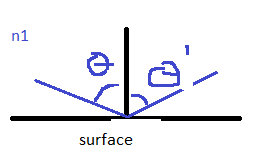
\includegraphics[width=\textwidth]{images/reflection.png}
		        \caption{Reflection: incident light beam gets reflected with the same angle relative to surface normal.}
		        \label{fig:reflection_def}
		    \end{subfigure}\hfill
		    \begin{subfigure}[t]{0.4\textwidth}
		        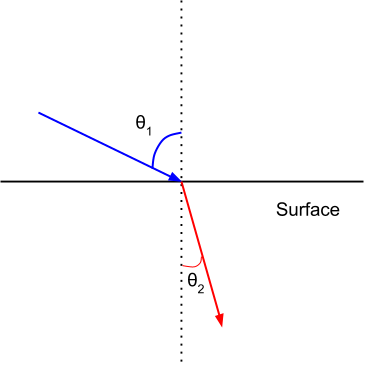
\includegraphics[width=\textwidth]{images/refraction.png}
		        \caption{Refraction: refracted light beam gets refracted according to Snell's law.}	
		        \label{fig:refracted_def}
		    \end{subfigure}%
		    
		    \begin{subfigure}[t]{0.5\textwidth}
		        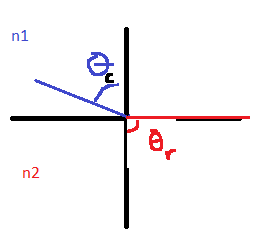
\includegraphics[width=\textwidth]{images/total_reflection.png}
		        \caption{Critical angle is reached when refracted angle is $90^\circ$.}
		        \label{fig:total_reflected_def}
		    \end{subfigure}
		    \caption{Reflection and refraction.}
	 		\end{figure}	
			
			\textbf{Refraction} is the change in direction of propagation of a wave when the wave passes from one medium into another with a different index of refraction. The angle of the reflected beam is shown in figure \ref{fig:refracted_def} is given by Snell's law:
			\begin{equation}
				n_1 \sin(\theta_1) = n_2 \sin(\theta_2)
			\end{equation}
				Where $n_1$ and $n_2$ are the indices of refraction of the media.
				
				\textbf{Total reflection} occurs when angle of the incident beam is larger than the critical angle:
				\begin{equation}
					\theta_c = \arcsin\left(\dfrac{n_2}{n_1}\right)
				\end{equation}
				
				
		\subsection{Bubble-light interaction}
			Since the smallest bubble radius (around 50-100 $\mu m$) is much larger than the wavelength of our light source (around 600 nm), diffraction within the air bubble can be neglected. Mie scattering effects are also only relevant for radii within the same order of magnitude as the wavelength (Demtroeder 2) so it can be neglected as well. Therefore, only refraction and reflection laws will be considered. 
			
			\begin{figure}
		    \centering
		    \begin{subfigure}[t]{0.5\textwidth}
		    		\centering
		        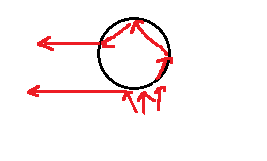
\includegraphics[scale=.5]{images/bubble_refraction.png}
		        \caption{Light beams inside a bubble. Reflected beams' intensities inside the bubble are described by Fresnel's law.}
		        \label{subfig:bubble_refraction}
		    \end{subfigure}%
		    \begin{subfigure}[t]{0.5\textwidth}
		    		\centering
		        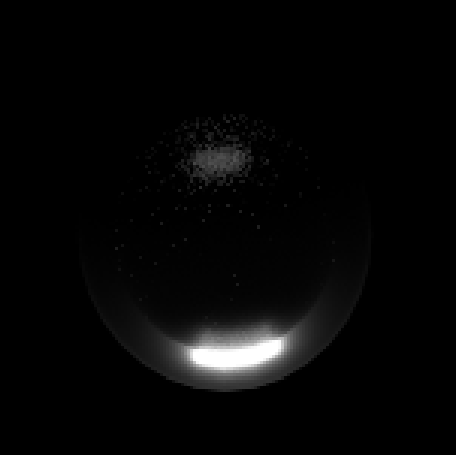
\includegraphics[scale=0.6]{images/bubble_simulation.png}
		        \caption{Simulated bubbles with ray tracing.}	
		        \label{subfig:bubble_simulation}
		    \end{subfigure}
		    
		    \caption{Interaction of a light bubble with light rays}
		    \label{fig:bubble_physics}
	 		\end{figure}	
			
			Figure \ref{subfig:bubble_refraction} shows refracted rays inside an air bubble. Since the outside medium (water) is more dense, total refraction occurs at the lower bubble boundary. Simulation in figure \ref{subfig:bubble_simulation} also shows that when a bubble is lit from bellow, two peaks can be observed. The lower peak is strong because it arises from total reflection on the lower bubble boundary, whereas the upper peak is much weaker. The second peak arises from internal (partial) reflections within the bubble and can be best explained by the Fresnel equations (Demtroeder 2). 
			The different peaks characteristics will be exploited by our proposed algorithm in order to compute the bubble's depth and radius.
			
			
	
	\section{Image processing}	\label{image_processing}
	In the following we represent an image as a two dimensional signal written as a matrix \textit{\textbf{g}}. $g_{m,n}$ denotes the pixel (i.e. picture element) at the \textit{m}-th row corresponding to the \textit{n}-th column. The chosen coordinate system is described in figure \ref{fig:coord_sys}. 
	
		\begin{figure}
		    \centering
		    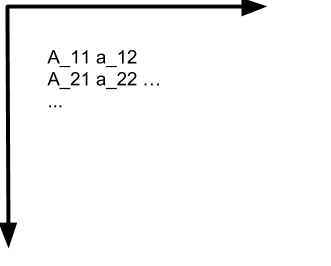
\includegraphics[scale=0.4]{images/coord_sys.png}
		    \caption{Notation and coordinate system}
		    \label{fig:coord_sys}
		\end{figure}
	
		\subsection{Fourier theory}
		The Fourier transform is an important image processing tool which is used to decompose an image into its since and cosine components. The output of the transformation represents the image in the Fourier or frequency domain, while the input image is the spacial domain. In the Fourier domain image, each point represents a particular frequency contained in the spatial domain image.
		The \textit{continuous} two-dimensional Fourier transform is defined as
		\begin{equation}
				\mathscr{F}\{ g(\mathbf{x})  \} = \hat{g}(\mathbf{k}) = 
				\int_{-\infty}^{\infty} g(\mathbf{x}) \text{exp}\left( -2 \pi \text{i} \mathbf{k}^T \mathbf{x}  \right) \text{d}\mathbf{x}
		\end{equation}
		and the inverse Fourier transform
		\begin{equation}
				\mathscr{F}^{-1}\{ \hat{g}(\mathbf{k}) \} = g(\mathbf{x}) =
				 \int_{-\infty}^{\infty} \hat{g}(\mathbf{k})
			\text{exp}\left( -2 \pi \text{i} \mathbf{k}^T \mathbf{x}  \right) \text{d}\mathbf{x}
		\end{equation}
		Where $\mathbf{x}$ and $\mathbf{k}$  are the two dimensional space and frequency vectors respectively. 
		
		Images however are discrete two dimensional signals, we therefore need to apply the \textit{Discrete} Fourier transform or DFT, defined as
		\begin{equation}
			\text{DFT}\{ g_{m,n} \} = \hat{g}_{u,v} = \dfrac{1}{MN} \sum_{m=0}^{M-1} \sum_{n=0}^{N-1}
			g_{m,n} \text{ exp} \left(  - \dfrac{2 \pi \text{i} m u}{M}  \right)
						\text{exp} \left(  - \dfrac{2 \pi \text{i} n u}{N}  \right)
		\end{equation}		 

		Similarly, the inverse 2-D DFT is defined as 
		
		\begin{equation}
		 \text{IDFT}\{\hat{g}_{u,v}\} = g_{m,n} = \sum_{m=0}^{M-1} \sum_{n=0}^{N-1} \hat{g}_{u,v}
			\text{ exp} \left(   \dfrac{2 \pi \text{i} m u}{M}  \right)
			\text{exp} \left(   \dfrac{2 \pi \text{i} n u}{N}  \right)
		\end{equation}
		
		
		\subsection{Convolution}
		Convolution is one of the most important operations in signal processing. Convolving two signals $g$ and $h$ produces a third signal that expresses how the shape of one is modified by the other. Formally, we define the continuous convolution as follows
		\begin{equation}
			(g \star h)(\mathbf{x}) = \int_{-\infty}^{\infty} 
			h(\mathbf{x}') g(\mathbf{x} - \mathbf{x}')
			\text{d}\mathbf{x}
		\end{equation}
		and the discrete two dimensional convolution as
		\begin{equation}
			g'_{m,n} = \sum_{m'=0}^{M-1} \sum_{n'=0}^{N-1}
			h_{m',n'} g_{m-m', n-n'}
		\end{equation}
		
		One important property of convolution is that we can express it as a multiplication in the Fourier domain. 
		\begin{equation}
		\mathscr{F}\{g \star h\} = N M \hat{h} \hat{g}
		\end{equation}
		This property, together with the fast Fourier implementation of the Fourier transform allows a fast computation of convolutions. 
		
		At the edge of the image, we typically extend the image with zero values (i.e. zero padding). This introduces an error when applying filters at the image border and we will mostly exclude the border when using filters (see chapter \ref{the_algorithm} for more details).
		
		\subsection{Smoothing}\label{sect:smoothing}
		Smoothing an image means convolving an image with a smoothing filter. A smoothing or averaging filters must ideally fulfill following conditions
		\begin{enumerate}
			\item Zero-shift: $\Im (\hat{h}(\mathbf{k})) = 0$
			\item Preservation of mean value: $\hat{h}(0) = 1 $
			\item Monotonous decrease: $ \hat{h}(k_1) \leq \hat{h}(k_2) $ for $ k_2 > k_2 $
			\item Isotropy: $\hat{h}(\mathbf{k}) = \hat{h}(| \mathbf{k} |)$
		\end{enumerate}
		
		In this work, we will be using Gaussian filters for one and two dimensional smoothing. Although Gaussian filters are not ideal, e.g. isotropy is violated for small standard deviations, it is still a good approximation for an ideal low pass filter. Computing the Fourier transform (for convolution) is also faster for a Gaussian filter. The $m$-th component of a one dimensional Gaussian filter mask can be obtained from the Gaussian function
		\begin{equation}
		G_{m} = \dfrac{1}{2 \pi \sigma^2} \text{ exp}
			 \left( 
			 	- \dfrac{(m-\mu)^2}{2 \sigma^2}
			 \right)
		\end{equation}
		Where $\mu$ is the mean, i.e. Gaussian peak's position and $\sigma$ is the standard deviation, i.e. peak's width.
		
		Figure \ref{fig:gauss_intro} show a Gaussian curve in one and two dimensions as well as the result of convolving an image with a Gaussian filter mask. Note how the image becomes blurry, i.e. large wave numbers have been suppressed.
		\begin{figure}
		    \centering
		    \begin{subfigure}[t]{0.3\textwidth}
		        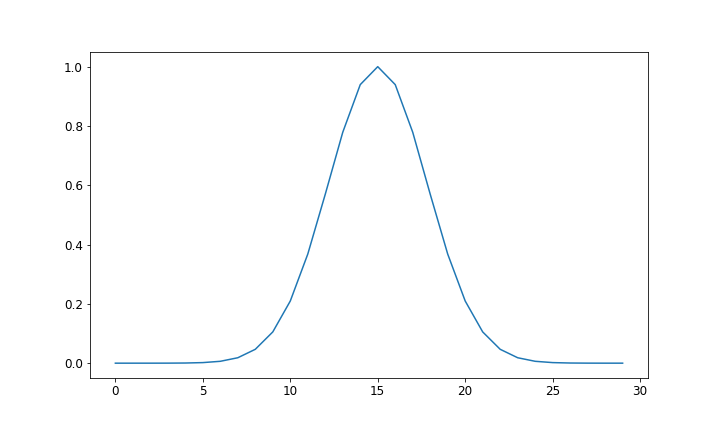
\includegraphics[width=\textwidth]{graphs/gauss_sigma_4.png}
		        \caption{1D Gaussian signal with $\mu=15$ and $\sigma=2$}
		    \end{subfigure}%
		    \begin{subfigure}[t]{0.3\textwidth}
		        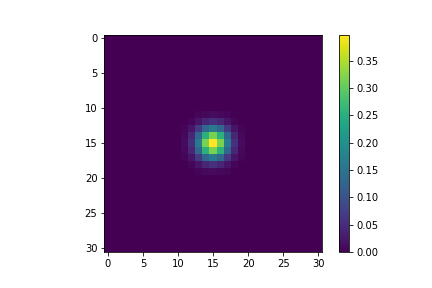
\includegraphics[width=\textwidth]{images/gauss_sigma_2.png}
		        \caption{2D Gaussian signal with $\mu_x = \mu_y = 15$ and $\sigma_x = \sigma_y = 4$}
		    \end{subfigure}
		    
		    \begin{subfigure}[t]{0.3\textwidth}
		        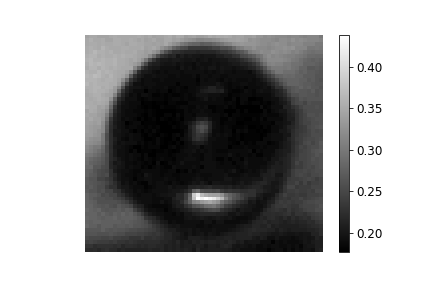
\includegraphics[width=\textwidth]{images/green_one.png}
		        \caption{Original image}
		    \end{subfigure}
			  \begin{subfigure}[t]{0.3\textwidth}
		        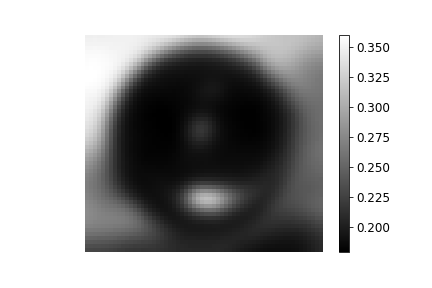
\includegraphics[width=\textwidth]{images/green_one_gaussian.png}
		        \caption{After convolution with 2D Gaussian mask}
		    \end{subfigure}
		    ~ %add desired spacing between images, e. g. ~, \quad, \qquad, \hfill etc. 
		    %(or a blank line to force the subfigure onto a new line)

		    \caption{Gaussian smoothing filter}
		    \label{fig:gauss_intro}
		\end{figure}




		\subsection{Edges and Derivation}
		\begin{figure}
			\centering
			\begin{subfigure}[t]{.4\linewidth}
				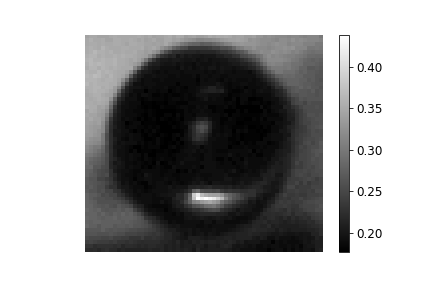
\includegraphics[scale=0.4]{images/green_one.png}
				\caption{Original bubble image}
			\end{subfigure}\hfill
			\begin{subfigure}[t]{.4\linewidth}
				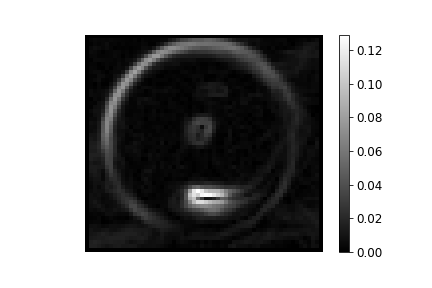
\includegraphics[scale=0.4]{images/green_one_sobel.png}
				\caption{Sobel filter filter applied.}
			\end{subfigure}
			
			\caption{Computing image derivative. Edges are detected by applying a derivative filter.}
			\label{fig:sobel_demo}
		\end{figure}
		An edge can be defined as a set of continuous pixel positions where an abrupt change of intensity (i.e. gray value) occurs. Therefore, edge detection is based on differentiation, where in discrete images differentiation is replaced by discrete differences that are mere approximation to differentiation. There is also the need to not only know where edges are, but also how strong they are.
		
		In continuous space, a partial derivative operation is defined as
		\begin{equation}
		 	\mathbf{\nabla} = \left[ \dfrac{\partial}{\partial x}, \dfrac{\partial}{\partial y} \right]
		\end{equation}
		and its corresponding Fourier transform is
		\begin{equation}
			\mathscr{F}\{\mathbf{\nabla}\} = 2 \pi \text{i} \mathbf{k}
		\end{equation}
		
		For the second derivative we need to consider all possible combinations of second order partial differential operators of a two dimensional signal. The resulting $2 \times 2$ matrix is called the Hessian matrix
		\begin{equation}
			\mathbf{H} = 
				\begin{bmatrix}
   \dfrac{\partial^2}{\partial x^2}       & \dfrac{\partial^2}{\partial x \partial y}\\
   \dfrac{\partial^2}{\partial y \partial x}       & \dfrac{\partial^2}{\partial y^2}\\
				\end{bmatrix}
				\label{eq:hessian_def}
		\end{equation}
		and its Fourier transform is
		
		\begin{equation}
			\mathscr{F}\{\mathbf{H}\} = -4 \pi^2 \mathbf{k}\mathbf{k}^T
		\end{equation}
		
		
		Edge detectors can be implemented as filters $h$ that operate on a two dimensional grid. 
%		
%		From the above equations we can derive the general properties for these filters:
%		\begin{enumerate}
%			\item Zero-shift: 
%				\begin{itemize}
%					\item $90^\circ$ phase shift for first order derivative, implying $ \Im\{ \hat{h} \} \neq 0$ and an antisymmetric filter mask, i.e $h_{-n} = -h_{n}$
%					\item a second order derivative operator must be symmetric in order to satisfy the zero shift property, i.e. $h_{-n} = h_{n}$
%				\end{itemize} 
%				
%			\item Suppression of mean value: $\hat{h}(k_i =0) \Leftrightarrow \sum_{\mathbf{n}}h_{\mathbf{n}} = 0$
%			
%			\item isotropy: For good edge detection, the edge detector's response must not depend on the direction of the edge. 
%				\begin{itemize}
%					\item first order derivative $\hat{h}(\mathbf{k}) = 
%											\pi \text{i} k_i \hat{b} (|\mathbf{k}|)$
%					\item second order derivative $\hat{h}(\mathbf{k}) = 
%											\pi^2 k_i^2 \hat{b} (|\mathbf{k}|)$
%				\end{itemize}
%				where $k_i$ denotes the wave number in the $i$-th direction and $b$ is an isotropic smoothing filter that fulfills the conditions
%				\begin{equation}
%					\hat{b}(\mathbf{0}) = 1, \hspace{1cm} \mathbf{\nabla}_k \hat{b}(|\mathbf{k}|) = \mathbf{0}
%				\end{equation}
%		\end{enumerate}
			
		In this work we will be using the Sobel filter masks as defined in equation (\ref{eq:sobel}) in order to compute derivatives in $x$ and $y$ directions. 
		\begin{equation}
			S_x =
			 \begin{bmatrix}
     				1	& 2 & 1 \\
    					0	 & 0 & 0 \\
    					-1	 & -2 & -1 \\
				\end{bmatrix},
			\hspace{2cm}
			S_y = 
				\begin{bmatrix}
     				1	& 0 & -1 \\
    					2	 & 0 & 2 \\
    					1	 & 0 & -1 \\
				\end{bmatrix}
			\label{eq:sobel}
			\end{equation}
		At each point in the image, the resulting gradient approximations can be combined to give the gradient magnitude image $S$ using:
		\begin{equation}
			S = \sqrt{(S_x \star G )^2 + (S_y \star G)^2}
			\label{eq:grad_sobel}
		\end{equation}

%		as well as the orientation $\theta$
%		\begin{equation}
%			\theta = \arctan \left(\dfrac{S_y \star G}{S_x \star G}\right)
%		\end{equation}

		where G is the input image. Figure \ref{fig:sobel_demo} shows the result of applying the derivation operator on an image. Note how edges have different magnitude depending on their strength. 
		
		
		\subsection{Orientation and Structure Tensor}
		\begin{figure} %fig:struct_tensor_intro
			\centering
			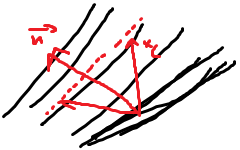
\includegraphics[scale=1]{images/structure_tensor_intro.png}
			\caption{Ideal local neighborhood described by a unit vector $\tilde{\mathbf{n}}$}
			\label{fig:struct_tensor_intro}
		\end{figure}
		Although derivation is useful to determine the gradient magnitude and its direction in an image, it doesn't tell us much about gradient directions in a specific neighborhood of a point. Figure \ref{fig:struct_tensor_intro} shows that in a neighborhood with ideal orientation gray values change in one direction only. Generally, the direction of local orientation can be denoted with a unit vector $\tilde{\mathbf{n}}$. If we orient the coordinate system along the principal directions, the gray values become a one dimensional function and a simple neighbourhood can be represented by
		\begin{equation}
			g(\mathbf{x}) = g(\mathbf{x}^T \tilde{\mathbf{n}})
		\end{equation}


%		The drawback of this representation however, is that it cannot distinguish between neighborhoods with constant values and isotropic orientation distribution. So if we define the optimum orientation as the orientation that shows the least deviations from the directions of the gradient, we can expressed it using the unit vector $\tilde{\mathbf{n}}$ as
%		\begin{equation}
%			\mathbf{\nabla}g^T \tilde{\mathbf{n}} = \cos[\angle(\mathbf{\nabla}g, \tilde{\mathbf{n}})]\\
%			\Leftrightarrow \\
%			\left( \mathbf{\nabla}g^T \tilde{\mathbf{n}} \right)^2 = 
%						 |\mathbf{\nabla}g|^2 \cos^2[\angle(\mathbf{\nabla}g, \tilde{\mathbf{n}})]
%		\end{equation}
%		We can see that this quantity is maximized when the orientation is along the unit vector $\tilde{\mathbf{n}}$, i.e. when $\mathbf{\nabla}g$ and $\tilde{\mathbf{n}}$ are either parallel or antiparallel. Therefore, the following integral is maximized in a local neighborhood:
%		\begin{equation}
%			\int w(\mathbf{x} - \mathbf{x'}) 
%								\left( 
%									 \mathbf{\nabla}g(\mathbf{x'})^T \tilde{\mathbf{n}}
%								\right)^2
%								\text{d}\mathbf{x'}
%			\label{eq:max_integral}
%		\end{equation}
%		where the window function $w$ determines the size and shape of neighborhood around a point $\mathbf{x}$ in which the orientation is averaged. 		
%		The maximization problem must be solved for each point $\mathbf{x}$, so we can write the maximization problem as follows:
%		\begin{equation}
%			\tilde{\mathbf{n}}^T \mathbf{J} \tilde{\mathbf{n}} \rightarrow \text{max}
%			\label{eq:max_prob}
%		\end{equation}
		
%		From equation \ref{eq:max_integral} and \ref{eq:max_prob} we can define \textbf{the structure tensor} as 

		From this principle we can derive the structure tensor (cite Jähne )
		\begin{equation} 
			\mathbf{J} = \int w(\mathbf{x} - \mathbf{x'}) 
								\left( 
									\mathbf{\nabla}g(\mathbf{x'}) \mathbf{\nabla}g(\mathbf{x'})^T
								\right)
								\text{d}\mathbf{x'}
		\end{equation}
		
		The $pq$-th component of this tensor is therefore given by
		\begin{equation}
			J_{pq} = \int_{-\infty}^{\infty} w(\mathbf{x} - \mathbf{x'}) 
							\left(
								\dfrac{\partial g(\mathbf{x'})}{\partial x'_p} \dfrac{\partial g(\mathbf{x'})}{\partial x'_q}
							\right)
							\text{d} \mathbf{x'}
			\label{eq:struct_tensor_pq}
		\end{equation}
		
%		Rotating equation \ref{eq:max_prob} into principle coordinate system yields:
%		\begin{equation}
%				\begin{bmatrix}
%    					 n_1' & n_2' \\
%				\end{bmatrix}
%				\begin{bmatrix}
%    					 J_{11}' & 0 \\
%    				  0 & J_{22} \\
%				\end{bmatrix}
%				\begin{bmatrix}
%    					 n_1' \\
%    				   n_2' \\
%				\end{bmatrix}
%				=
%				J' = J_{11}'n_1' + J_{22}'n_2' \rightarrow \text{max}
%		\end{equation}					
%		We can see that $J'$ is maximized for $\tilde{\mathbf{n}} = [1 \hspace{0.3cm} 0]^T$ (assuming $J_{11}' > J_{22}'$), where the maximum value is $J_{11}$, so solving this problem is equivalent to solving the eigenvalue problem for $\mathbf{J}$. We can then extract the orientation $\theta$ as follows:
%		\begin{equation}
%			\begin{bmatrix}
%    					 \lambda_1 & 0 \\
%    					 0		& \lambda_2
%				\end{bmatrix}
%				=
%				\begin{bmatrix}
%    					 \cos(\theta) & \sin(\theta) \\
%    				  	-\sin(\theta) & \cos(\theta) \\
%				\end{bmatrix}
%				\begin{bmatrix}
%    					 J_{11} & J{12} \\
%    				  J_{21} & J_{22} \\
%				\end{bmatrix}
%				\begin{bmatrix}
%    					 \cos(\theta) & -\sin(\theta) \\
%    				  	\sin(\theta) & \cos(\theta) \\
%				\end{bmatrix}
%		\end{equation}
% Using trigonometric identities, this yields 
	
		Orientation can be obtained from	
		\begin{equation}
			\tan(2\theta) = \dfrac{2 J_{12}}{J_{11} - J_{22}}
		\end{equation}
	
		The importance of the structure tensor stems from the fact the eigenvalues (which can be ordered $\lambda_1 \geq \lambda_2 \geq 0$ and the corresponding eigenvectors summarize the distribution of the gradient within the window defined by $w$. Table \ref{tab:struc_tensor_interp} shows how eigenvalues can be interpreted.
		
		\begin{table}
		
			\begin{tabular}{|l|l|l|p{5cm}| }
			\hline 
			\textbf{Condition} & \textbf{Rank(J)} & \textbf{Description }\\ 
			\hline 
			$ \lambda_1 = \lambda_2 = 0$  & 0 & Local neighborhood  has constant values\\ 
			\hline 
			$\lambda_1 \geq 0, \lambda_2 = 0 $ & 1 & The local neighborhood is a simple neighborhood \\
																				&  		& with ideal orientation.  \\ 
			\hline
			 $\lambda_1 \geq 0, \lambda_2 \geq 0 $ & 2 & Gray values change in all directions \\
			\hline
			\end{tabular} 
			
			\caption{Interpretation of the eigenvalues of a structure tensor}
			\label{tab:struc_tensor_interp}
		\end{table}
		
		
		For discrete images, we use Sobel filters as defined in equation \ref{eq:sobel} for derivation and a Gaussian smoothing mask introduced in section \ref{sect:smoothing}. Computing the elements of a structure tensor for an image $G$ therefore requires following steps:
		\begin{enumerate}
			\item $G_x = S_x \star G$ \\
						$G_y = S_y \star G$
			\item $J_{11} = M \star (G_x \times G_x)$ \\
						 $J_{12} = J_{21} = M \star (G_x \times G_y)$ \\
						 $J_{22} = M \star (G_y \times G_y)$
		\end{enumerate}
		Where $M$ is a smoothing mask and $S_x$ and $S_y$ are derivation masks in $x$ and $y$ directions respectively.

		Figure \ref{fig:struct_tensor_demo} shows an extracted orientation from a bubble image using the structure tensor.
		
		\sidecaptionvpos{figure}{t}
		\begin{SCfigure}
			\centering
			\caption{Orientation angle using sobel filters for derivation and a Gaussian mask with $\sigma =1$ for smoothing.}		
			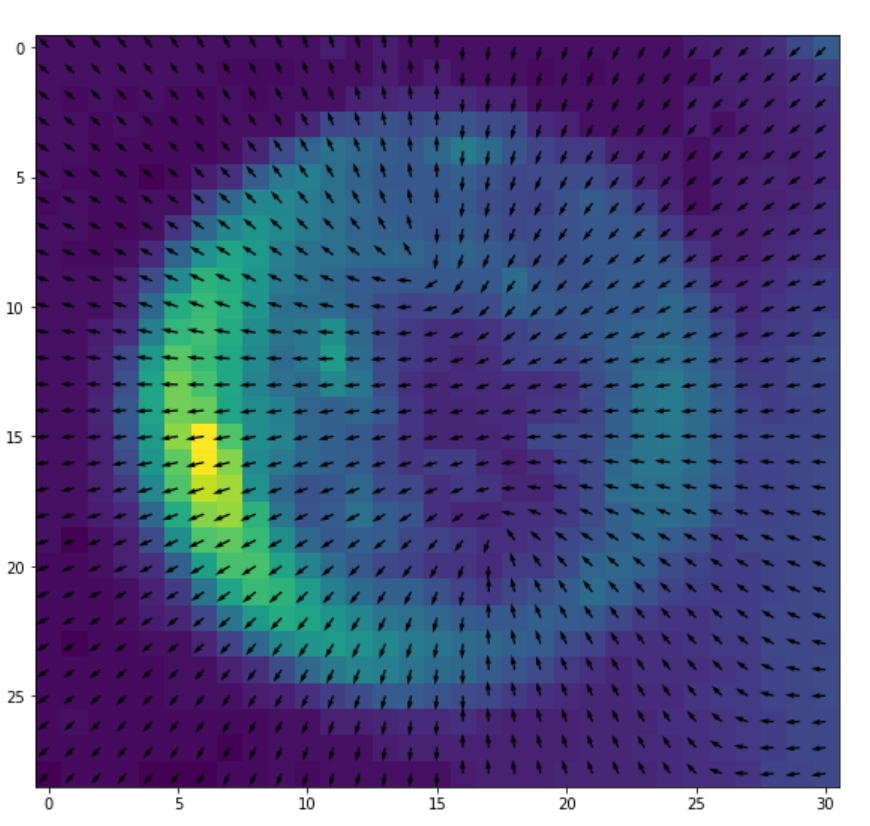
\includegraphics[scale=0.4]{images/structure_tensor_demo.png}
			\label{fig:struct_tensor_demo}
		\end{SCfigure}
		
	
	\section{The object detection problem}\label{the_object_detection_problem}
	
	Our proposed algorithm recognizes bubbles (classification) in an image and estimates their respective centers and radii (localization). This problem of classification and localization is known as the object detection problem. Figure \ref{fig:obj_detec_intro} shows a typical output of an object detection algorithm. 
	
		\begin{figure}
			\centering
			\begin{subfigure}[t]{0.4\linewidth}
				\centering
				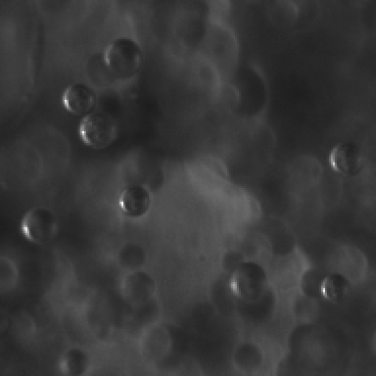
\includegraphics[scale=.4]{images/object_detection_intro_1.png}
				\caption{Input image.}
			\end{subfigure}
			\begin{subfigure}[t]{0.4\linewidth}
				\centering
				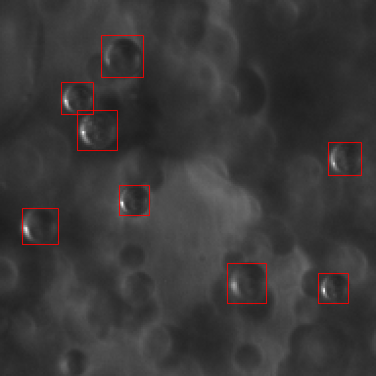
\includegraphics[scale=.4]{images/object_detection_intro_2.png}
				\caption{Output format.}
			\end{subfigure}
			\caption{Output of an object detection algorithm. Bounding boxes around correctly classified bubbles are returned.}
			\label{fig:obj_detec_intro}
		\end{figure}
	
	There has been a lot of progress in this field thanks to deep learning algorithms (see next section) that rely on training a relatively complex model a large amount of annotated data. The sate of the art algorithms include region based methods such as Faster R-CNN (cite fasterRcnn), where many candidate regions are first extracted and then classified and single evaluation methods such as YOLO (cite YOLO) where bounding boxes and class probabilities are estimated with one single neural network in a single evaluation. Although these algorithms perform very well on typical photographs and support between 1000 and 9000 different classes, applying them to our problem yields very bad results (see chapter \ref{the_algorithm}). We still however opt for a machine learning based approach for the classification part, and then perform localization with more straightforward methods.
		
		\subsection{Classification}\label{machine_learning}
		In our work, we use machine learning techniques mainly for signal classification purposes. For instance, both of the proposed algorithms rely on binary classification using a random forest classifier and a convolutional neural network. In this section, we explain the principle behind machine learning and the main idea behind the chosen model. A more thorough argumentation about the chosen architecture and model-specific parameters is discussed in chapter \ref{the_algorithm}.

		Machine learning is commonly defined as the practice of using algorithms to parse data, learn from it, and then make a determination or prediction about something. In our case, this means training our model with a large number of bubble and background instances, in order to predict whether a given signal corresponds to a bubble or not. Figure \ref{fig:machine_learning_intro} summarizes the principle behind machine learning. 
		
		\begin{figure}
			\centering
			\begin{subfigure}[b]{0.55\textwidth}
				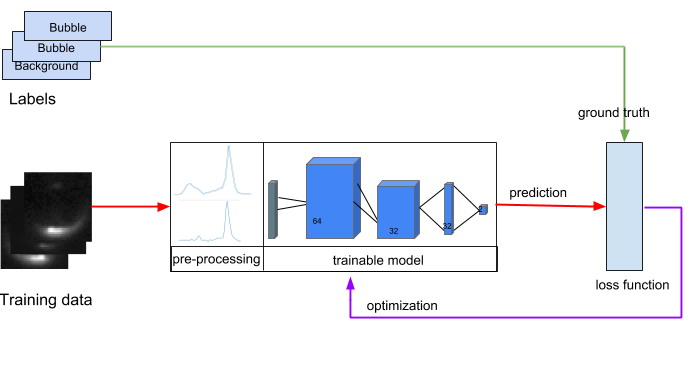
\includegraphics[scale=.5]{images/training_intro.png}
				\caption{Training}
			\end{subfigure}
			\begin{subfigure}[b]{0.55\textwidth}
				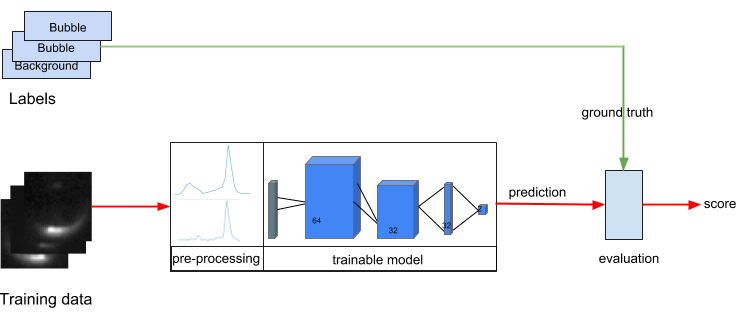
\includegraphics[scale=.5]{images/testing_intro.png}
				\caption{Testing}
			\end{subfigure}
			\caption{Training and testing in machine learning}
			\label{fig:machine_learning_intro}
		\end{figure}				
		
		
		\subsubsection{Terminology}
			\begin{itemize} 
				\item \textbf{Training} is changing the model's parameters based on the model's output. Training is also referred to as optimization. When training data is annotated, we speak of supervised training. 
				\item \textbf{Testing} is assigning a score to a trained model based on annotated testing data. The score is typically by an evaluation criteria and is independent of the model itself. 
				\item \textbf{Validation} is a form of testing, so it assigns a score to a trained model. Validation is needed when we want to choose the best model among some trained candidate models based on their testing performance. Since changing a parameter of the algorithm (in this case the whole model) based on the output is equivalent to training by definition, we need an independent data set to compute the final score of the algorithm, i.e. validation data. 
			\end{itemize}				
			
		\subsubsection{Logistic Regression Classifier}
			Logistic regression is despite its name a linear model for classification, where the probabilities describing the possible outcome of a single trial are modeled using a logistic function (sigmoid curve):
			\begin{equation}
				lr(x) = \dfrac{A}{1 + e^{-k (x-x_0)}}
			\end{equation}
		where $x_0$ is the x-value of the sigmoid's midpoint, $A$ is the curve's maximum value and k is the steepness of the curve. This model is very simple and can be trained with relatively few data points. Its main drawback is its inability to generalize to complex data with high number of features. We make use of this classifier as a preprocessing step to generate training data for the more demanding convolutional neural network. 
		
		\subsubsection{Random Forest Classifier}\label{rand_forest_class}
			Random forest classifiers operate by constructing a multitude of decision trees at training time and outputting the class that is the mode of the classes (cite Ho, Tin Kam 1995). So random forest is an ensemble method in which a classifier is constructed by combining several different independent base classifiers. Their main advantage over a simple decision tree is the ability to describe the data well without overfitting. 			
			This method is well suited for small sized and balanced data set, given the chosen features describe the data well. It also allows an estimation of feature importance in the classification, something that neural networks are known to be lacking. Its main drawback is its tendency to generate deep trees during training, which makes evaluation computationally expensive. See (cite Pattern Recognition buch 2016) for a more in depth description of random forests. 
			
		\subsubsection{Convolutional Neural Network}
			First introduced by (cite AlexNet), a convolutional neural networks, or CNN is a class of deep, feed-forward artificial neural networks. Convolutional networks were inspired by biological processes in that the connectivity pattern between neurons resembles the organization of the animal visual cortex. Individual neurons activate only when stimulated in a restricted region of the visual field known as the receptive field. The receptive fields of different neurons partially overlap such that they cover the entire visual field. CNNs are known for their ability to generalize well to large, mutlidimensional data. They also require very little preprocessing. For instance, neural networks learn the filters needed to extract features using back propagation (i.e. stochastic gradient descent) to optimize convolutional and dense layers within the neural network. This eliminates the need to first compute features and then pass them to the classifier as is done by classical machine learning algorithms such as random forests.
			
			The drawback of using a CNN is the need of a large amount of data and computational power for proper training. It is also not possible to extract feature importance from a trained CNN, which makes CNNs resemble black boxes that are hard to interpret.  
			 (cite Neural Network Methods for Natural Language Processing) explain CNNs in more details.
		
		\subsection{Evaluation Criteria: IoU@p-mAP}
		  We evaluate our object detection algorithm using the \textit{intersection over union at $p$ mean average precision} criteria as explained in figure \ref{fig:iou_def}. As the  name suggests, we compute the area of intersection between the predicted and the ground truth bounding boxes and then divide it by union area of the two boxes. This means that IoU = 1 corresponds to a perfect prediction and IoU = 0 is a complete miss (assuming original images were annotated perfectly). So we choose a threshold $p$, so that IoU $>= p$ or simply IoU@p corresponds to a correct prediction or \textit{true positive}. 		  

		\begin{figure}
			\centering
			\includegraphics[scale=.5]{images/iou_def.png}
			\caption{Definition of intersection over union. Green represents predicted bounding box and red is the ground truth. Areas are drawn in blue}
			\label{fig:iou_def}
		\end{figure}				  
		  
		  \textit{Mean average precision} refers to the average of the maximum precision at different recall values, where \textbf{precision} and \textbf{recall} are defined as
		  \begin{equation}
		  	precision = \dfrac{True \hspace{.1cm} Positive}{True \hspace{.1cm}  Positive + False \hspace{.1cm}  Positive}
		  \end{equation}
		  \begin{equation}
		  	recall = \dfrac{True \hspace{.1cm}  Positive}{True \hspace{.1cm}  Positive + False \hspace{.1cm}  Negative}
		  \end{equation}

		From the above definition it becomes clear that precision measures how accurate the predictions are and recall measures how well all the positives can be found.
		
		Since our algorithm performs binary classification, \textit{mean average precision} is equivalent to \textit{average precision} in our case. 
		
		\textbf{Note:} This criteria only shows how well the algorithm is at detecting bubbles from an image, and does not necessarily make a strong statement on how well the measurement technique as a whole performs at estimating bubble size distributions in a water. 
		
		 



































